\section{The coefficients and the quadratic identities}

The construction has two parts: explicit real coefficients define the
matrix $\mathsf B$, and a finite Fourier transform proves its quadratic
identities.
Fix an odd integer $n\geq3$, put $G=\Z/n\Z$, and set
\[
 d=\frac{n+\sqrt{n^2+4}}2,\qquad \delta=-d^{-1},\qquad
 \tau=\delta-1,\qquad
 \omega_1=d+1,\qquad \omega_2=1+d^{-1}.
\]
The relations used below are
\[
 \delta^2=n\delta+1,\qquad \omega_1-\omega_2=n,\qquad
 \Omega:=\omega_1+\omega_2=\omega_1\omega_2,\qquad
 \omega_1/\omega_2=d,\qquad \tau=-\omega_2.
\]
Since $n^2<n^2+4<(n+1)^2$, the numbers $d$ and $\omega_2$ are
irrational. In particular,
$(\omega_1\Z+\omega_2\Z)\cap\Z=n\Z$: writing
$r\omega_1+s\omega_2=rn+(r+s)\omega_2$ shows that an integer value
requires $r+s=0$.

\subsection{Double-sine samples and the coefficient matrix}\label{coeff}

Let $\gamma(z)=\gamma^{(2)}(z;\omega_1,\omega_2)$ be the hyperbolic
gamma function in the normalization of \cite{BSS}. On
$0<\Re z<\Omega$ it is defined by the absolutely convergent integral
\[
 \gamma(z)=\exp\left\{-\int_0^\infty
 \left[\frac{\sinh((2z-\Omega)t)}
 {2\sinh(\omega_1t)\sinh(\omega_2t)}
 -\frac{2z-\Omega}{2\omega_1\omega_2t}\right]\frac{dt}{t}\right\},
\]
and is continued by its shift identities. The subtraction is kept
inside the integral to cancel the singularity at zero. The identities
we use, understood as identities of meromorphic functions, are
\begin{align}
 \gamma(z+\omega_1)&=2\sin(\pi z/\omega_2)\gamma(z),&
 \gamma(z+\omega_2)&=2\sin(\pi z/\omega_1)\gamma(z),
 \label{foundation:shifts}\\
 \gamma(z)\gamma(\Omega-z)&=1,&
 \Res_{z=0}\gamma(z)&=\frac{\sqrt\Omega}{2\pi}.
 \label{foundation:reflection}
\end{align}
Its poles are $-r\omega_1-s\omega_2$ and its zeros are
$\Omega+r\omega_1+s\omega_2$, for integers $r,s\geq0$.
They are simple because $\omega_1/\omega_2=d$ is irrational.
The integral gives positivity on $(0,\Omega)$, and the shifts give
reality on the real axis away from poles. Taking the first shift
identity at $z=0$ by a limit gives
$\gamma(\omega_1)=\sqrt\Omega/\omega_2=\sqrt d$; reflection gives
$\gamma(\omega_2)=1/\sqrt d$. Thus, for
$F(z)=1/\gamma(\omega_2+z)$,
\[
 F(0)=\sqrt d,\qquad F(z)F(n-z)=1,\qquad
 F(-a)F(a)=(-1)^{a+1}\quad(a\in\Z\setminus\{0\}).
\]
We have the following integer shift relation:
\begin{equation}\label{foundation:shift}
  F(a+n) = (-1)^{a+1}F(a)\quad(a\in\Z\setminus\{0\}).
\end{equation}
The excluded sample has the separate value $F(n)=1/\sqrt d$.
The poles of $F$ start at $\omega_1>n$ and its zeros at
$-\omega_2<-1$; hence the samples used to define the coefficients
are finite and nonzero.

Define the nonzero real coefficients
\begin{equation}\label{foundation:coefficients}
 W_0=-1,\qquad
 W_a=-(-1)^{a(a+n)/2}\frac{F(a)}{\sqrt d}
 \quad(1\leq a<n).
\end{equation}
Here the displayed integers specify the representatives of $G$.
In particular,
\begin{equation}\label{foundation:reciprocal-products}
 W_aW_{-a}=\delta\qquad(a\in G\setminus\{0\}).
\end{equation}
The matrix and its rescaling are
\begin{equation}\label{foundation:core}
 \mathsf B_{a,b}=
 \begin{cases}
  W_aW_{b-a}/W_b,&b\ne0,\\
  -1+\tau\ind{a=0},&b=0,
 \end{cases}
 \qquad \mathsf A_{a,b}=\tau^{-1}\mathsf B_{a,b}.
\end{equation}
Thus $\mathsf B_{0,0}=\delta-2$, and every other entry on either
axis or the diagonal equals $-1$. The reciprocal product identity
\eqref{foundation:reciprocal-products} also gives the order-three symmetry
\begin{equation}\label{foundation:rotation}
 \mathsf B_{a,b}=\mathsf B_{b-a,-a}.
\end{equation}

\emph{Bounds and contour values.} Since we will be working with various contour integrals containing multiple copies of hyperbolic gamma functions, we discuss the general ideas here and mention some subtleties involved.
The vertical asymptotics of \cite[Section~1]{BSS} give
\[
 \log|\gamma(x+it)|
 =\frac{\pi(x-\Omega/2)}{\omega_1\omega_2}|t|+O(1).
\]
In particular, for fixed real $c$,
\[
 \left|\frac{\gamma(x+it+c)}{\gamma(x+it)}\right|
 \leq C e^{\pi c|t|/(\omega_1\omega_2)}
 \quad(|t|\geq T).
\]
Both estimates are uniform for $x$ in a bounded interval.
Here $\omega_1\omega_2=\Omega$. The first estimate
also supplies bounds locally uniform in complex shifts: their real
and imaginary parts remain bounded on compact parameter sets.
Consequently a strict exponential decay margin for any gamma product
below persists in a parameter neighbourhood.

For a parameter-dependent integral with designated left and right pole
families, we work on open domains where opposite families do not meet
and the infinite tails have a locally uniform bound $Ce^{-c|\Im z|}$,
$c>0$. The pole families below are finite unions of translates of
one-sided period lattices. Locally one can keep a pole-free separating
contour fixed, agreeing with a vertical line outside a compact set.
The gamma factors are jointly holomorphic away from their poles;
compactness bounds the finite part of this contour and the exponential
estimate bounds its tails. Cauchy's estimates then justify
differentiation under the integral, giving holomorphy in the parameter.
Relative to an upward pole-free line, the separating
integral is the line integral plus $2\pi i$ times the residues of
left poles to its right, minus $2\pi i$ times the residues of right
poles to its left. These sums are finite. With the measure $dz/i$,
the correction factors are $2\pi$ instead.
Colliding poles of the same family are enclosed together by a fixed
loop; its integral remains holomorphic and represents the full sum
of their residues, including the residue at a merged pole. This
description also proves local holomorphy of the corrected line value.
If the chosen line meets a pole, move it and adjust the residue sums.

\subsection{The Fourier transform of a column of the coefficient matrix}
\begin{lemma}[Fourier transform]\label{foundation:column-fourier}
Write $u_p(a)=\mathsf B_{a,p}$. For $1\leq h<n$ and $k\in G$, define
\[
 \widehat u_h(k)=\sum_{a\in G}u_h(a)e^{-2\pi ika/n},
 \qquad
 \theta\equiv\frac{2\pi k}{n}+\pi(h-1)\pmod{2\pi},
 \quad -\pi\leq\theta\leq\pi.
\]
Then
\begin{equation}\label{fd:fourier}
 \widehat u_h(k)
 =-\omega_2 e^{-ih\theta/2}
   \gamma\left(\frac{\Omega+h}{2}-\frac{\Omega\theta}{2\pi}\right)
   \gamma\left(\frac{\Omega+h}{2}+\frac{\Omega\theta}{2\pi}\right).
\end{equation}
\end{lemma}

\begin{proof}
We choose a kernel whose integer residues give the summands of
$\widehat u_h(k)$, up to a common normalization and one correction
at $a=h$. Set
\[
 R_h(z)=\frac{F(z)}{F(z-h)},\qquad
 K_h(z)=\frac{\pi e^{-i\theta z}R_h(z)}{\sin\pi z}.
\]
At the integer samples, including $a=0,h$, the coefficient formula gives
\begin{equation}\label{foundation:sample}
 u_h(a)+\omega_2\ind{a=h}
 =\frac{(-1)^{h(a+1)}}{\sqrt d\,F(h)}R_h(a)
 \qquad(0\leq a<n).
\end{equation}
The ratio $R_h$ is holomorphic at these samples, and the residue of
$\pi/\sin\pi z$ at $z=a$ is $(-1)^a$. Consequently
\[
 \Res_{z=a}K_h(z)=(-1)^a e^{-i\theta a}R_h(a).
\]
Put $c_h=(-1)^h/(\sqrt d\,F(h))$. Since the choice of $\theta$ gives
$e^{-i\theta a}=(-1)^{a(h-1)}e^{-2\pi ika/n}$, equation
\eqref{foundation:sample} therefore gives
\[
 c_h\Res_{z=a}K_h(z)
 =\bigl(u_h(a)+\omega_2\ind{a=h}\bigr)e^{-2\pi ika/n}.
\]
Summing over the representatives $a=0,\ldots,n-1$ yields
\[
 \widehat u_h(k)
 =c_h\sum_{a=0}^{n-1}\Res_{z=a}K_h(z)
       -\omega_2e^{-2\pi ikh/n}.
\]
It remains to evaluate this integer residue sum.

\emph{The difference of the kernels.}
Put $\alpha=1/\omega_1$ and $\beta=1/\omega_2$, so
$\alpha+\beta=1$. Applying the shift identities and
\[
 (-1)^h\sin(\pi\alpha z)\sin(\pi\beta(z-h))
 -\sin(\pi\beta z)\sin(\pi\alpha(z-h))
 =\sin(\pi\alpha h)\sin\pi z
\]
gives
\begin{equation}\label{foundation:kernel-difference}
 K_h(z+n)-K_h(z)
 =-4\pi\sin(\pi h/\omega_1)e^{-i\theta z}\gamma(-z)\gamma(z-h).
\end{equation}

\emph{The residue rectangle.}
Let $L=\lfloor h/\omega_2\rfloor$ and choose
$\sigma=-\varepsilon$, where
$0<\varepsilon<\min\{1,(L+1)\omega_2-h\}$.
In the strip $\sigma<\Re z<\sigma+n$ (Figure~\ref{fig:contour}),
the poles of $K_h$ are the integers $0,\ldots,n-1$ from the cosecant
and $p_\ell=h-\ell\omega_2$ for $1\leq\ell\leq L$ from the
denominator of $R_h$.
The first pole of $F$ is at $\omega_1>n$, so the numerator of $R_h$ contributes
none. Irrationality of $\omega_2$ excludes coincident poles, and
$K_h(z+n)$ is regular at the additional poles $p_\ell$.
Indeed $p_\ell+n$ is not an integer. A numerator pole there would put
$h$ in $(\omega_1\Z+\omega_2\Z)\cap\Z=n\Z$, contrary to $0<h<n$.
A denominator zero would give
$n-\ell\omega_2=-r\omega_1-(s+1)\omega_2$, or
$(r+1)n=(\ell-r-s-1)\omega_2$, for $r,s\geq0$; irrationality makes
this impossible.
\begin{figure}
  \centering
  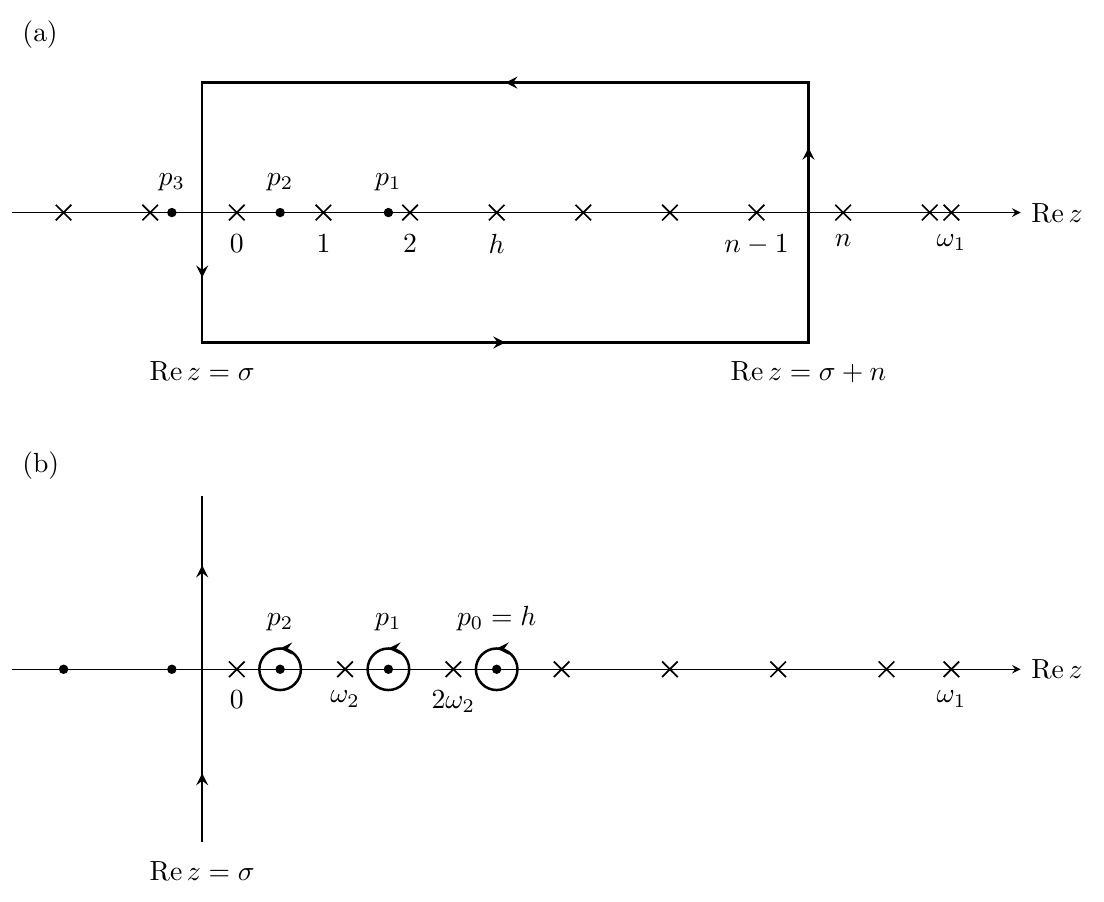
\includegraphics[width=0.7\linewidth]{plots/contour_lemma21.png}
  \caption{Contours for \eqref{foundation:rectangle}: (a) the residue rectangle, whose vertical sides are compared using \eqref{foundation:kernel-difference}; (b) the contour for $I_{\rm sep}$.}
  \label{fig:contour}
\end{figure}


The vertical ratio bound gives
\[
 |R_h(x+it)|=O(e^{-\pi h|t|/\Omega})
\]
uniformly on the closed strip. Since
$|\sin\pi(x+it)|^{-1}=O(e^{-\pi|t|})$ and
$|e^{-i\theta(x+it)}|\leq e^{\pi|t|}$, the same decay bound holds
for $K_h$. Hence its horizontal integrals vanish and its vertical
integrals converge, even at $|\theta|=\pi$.

Write $p_0=h$ and set
\[
 r_\ell=\Res_{z=p_\ell}
       e^{-i\theta z}\gamma(-z)\gamma(z-h),\qquad
 I_\sigma=\int_{\sigma-i\infty}^{\sigma+i\infty}
       e^{-i\theta z}\gamma(-z)\gamma(z-h)\frac{dz}{i}.
\]
Reflection and the ratio bound give
\[
 |\gamma(-x-it)\gamma(x+it-h)|
 =\left|\frac{\gamma(x+it-h)}{\gamma(x+it+\Omega)}\right|
 =O(e^{-\pi(1+h/\Omega)|t|}).
\]
Thus $I_\sigma$ converges uniformly for $|\theta|\leq\pi$.
The pole $p_0=h$ of the two-gamma integrand is already among the
integer poles of $K_h$; $R_h$ itself is regular there.
The residue theorem and \eqref{foundation:kernel-difference} yield
\begin{equation}\label{foundation:rectangle}
 \sum_{a=0}^{n-1}\Res_{z=a}K_h(z)
 =-2\sin(\pi h/\omega_1)I_\sigma
  -4\pi\sin(\pi h/\omega_1)\sum_{\ell=1}^{L}r_\ell.
\end{equation}

\emph{The integral evaluation and cancellation.}
Choose an upward separating contour, agreeing with the line
$\Re z=\sigma$ outside a compact set, which puts the poles of
$\gamma(z-h)$ on its left and those of $\gamma(-z)$ on its right
(Figure~\ref{fig:contoursep}). Write $I_{\rm sep}$ for its integral
with integrand $e^{-i\theta z}\gamma(-z)\gamma(z-h)$ and measure
$dz/i$. The two-gamma Fourier integral \cite[Eq.~(2.17)]{BSS}, with shifts
$-h,0$ and parameter
$\alpha_{\rm BSS}=(\Omega+h-\Omega\theta/\pi)/2$, gives
\begin{align}
 I_{\rm sep}
 &=\sqrt\Omega\,e^{-ih\theta/2}\gamma(-h)
   \gamma\left(\frac{\Omega+h}{2}-\frac{\Omega\theta}{2\pi}\right)
   \gamma\left(\frac{\Omega+h}{2}+\frac{\Omega\theta}{2\pi}\right),
   \label{foundation:beta}\\
 I_{\rm sep}&=I_\sigma+2\pi\sum_{\ell=0}^{L}r_\ell.
   \label{foundation:continued-contour}
\end{align}
\begin{figure}
  \centering
  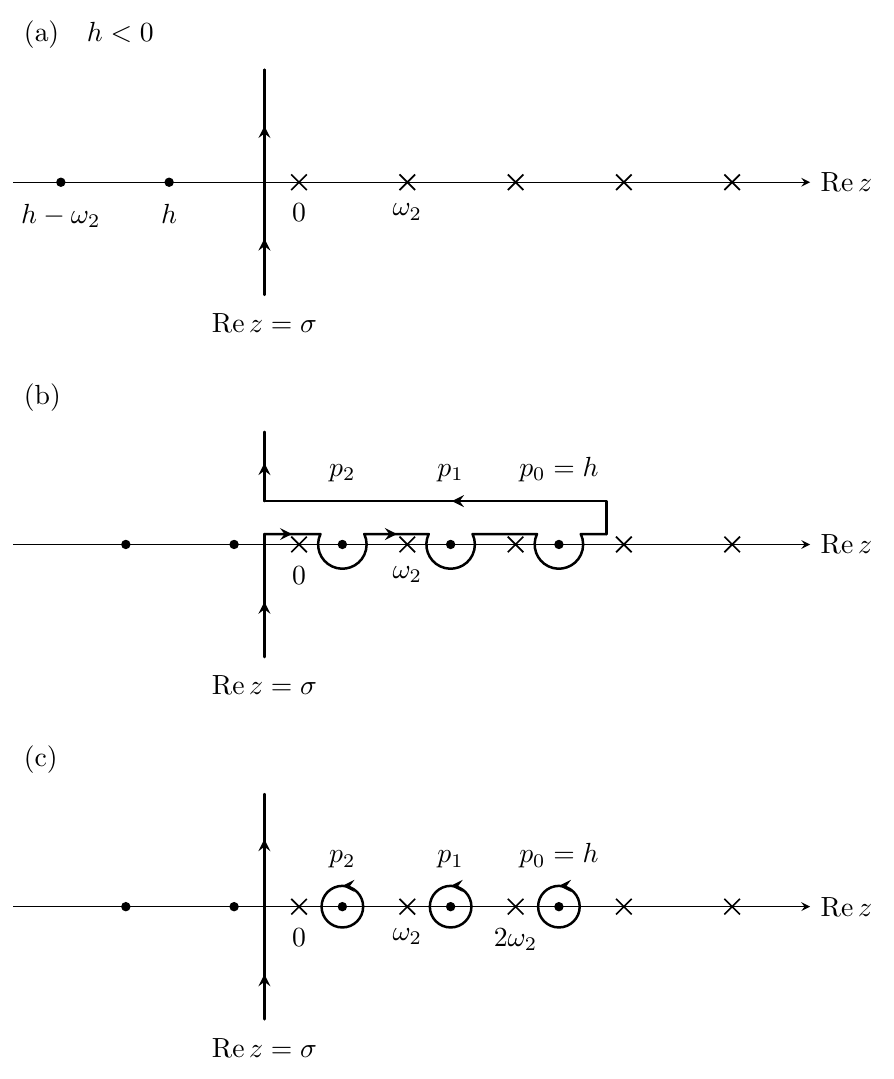
\includegraphics[width=0.7\linewidth]{plots/contour_isep.png}
  \caption{The separating contour as we vary $h$.}
  \label{fig:contoursep}
\end{figure}
To justify the continuation, first fix $|\theta|<\pi$ and replace
$h$ by a complex parameter $h'$. Its domain is the connected open set
\[
 U_\theta=\{h'\in\C:\Re h'>\Omega(|\theta|/\pi-1)\}
 \setminus(\omega_1\Z_{\geq0}+\omega_2\Z_{\geq0}).
\]
The inequality is exactly the strict decay condition for the
two-gamma integrand; the deleted discrete set is exactly the set of
opposite-pole collisions. Choose a real
$h_0\in(\max\{-1,\Omega(|\theta|/\pi-1)\},0)$ and a line
$h_0<\sigma_0<0$, independently of the final line $\sigma$.
Near $h_0$ this line separates the families and the BSS formula
applies directly. The contour prescription above gives a holomorphic
integral on $U_\theta$; its displayed gamma evaluation is also
holomorphic there, since $-h'$ avoids the pole lattice and the other
two arguments have positive real parts. The identity theorem proves
\eqref{foundation:beta} throughout $U_\theta$, in particular at
$h$: an integer $0<h<n$ cannot lie in the period lattice.
At this parameter the left poles to the right of $\sigma$ are exactly
$p_0,\ldots,p_L$, and there are no crossed right poles. The residue
prescription therefore gives \eqref{foundation:continued-contour}.
Finally let $\theta\to\pm\pi$ at fixed $h>0$. The bound for
$I_\sigma$ is uniform, the finitely many residue terms are continuous,
and the gamma arguments at the endpoints, $h/2$ and $\Omega+h/2$,
are positive. This proves both formulas at the endpoint frequencies.

Substituting \eqref{foundation:continued-contour} into
\eqref{foundation:rectangle} cancels all residues $r_\ell$ with
$\ell\geq1$ and gives
\[
 \sum_{a=0}^{n-1}\Res_{z=a}K_h(z)
 =-2\sin(\pi h/\omega_1)I_{\rm sep}
       +4\pi\sin(\pi h/\omega_1)r_0.
\]
The remaining residue and normalization are
\[
 r_0=\frac{\sqrt\Omega}{2\pi}e^{-i\theta h}\gamma(-h),\qquad
 2\sin(\pi h/\omega_1)\gamma(-h)=(-1)^hF(h),\qquad
 \frac{\sqrt\Omega}{\sqrt d}=\omega_2.
\]
Returning to the residue formula for $\widehat u_h(k)$ at the start
of the proof, and using \eqref{foundation:beta}, we obtain
\begin{align*}
 \widehat u_h(k)
 &=-2c_h\sin(\pi h/\omega_1)I_{\rm sep}
     +4\pi c_h\sin(\pi h/\omega_1)r_0-\omega_2e^{-2\pi ikh/n}\\
 &=-\omega_2e^{-ih\theta/2}
   \gamma\left(\frac{\Omega+h}{2}-\frac{\Omega\theta}{2\pi}\right)
   \gamma\left(\frac{\Omega+h}{2}+\frac{\Omega\theta}{2\pi}\right)\\
 &\qquad+\omega_2\bigl(e^{-i\theta h}-e^{-2\pi ikh/n}\bigr).
\end{align*}
Since $h(h-1)$ is even, the frequency congruence implies
$e^{-i\theta h}=e^{-2\pi ikh/n}$. Thus the $r_0$ contribution cancels
the diagonal sample correction, leaving exactly the stated Fourier
transform \eqref{fd:fourier}.
\end{proof}

\subsection{Fourier inversion gives the quadratic identities}

\begin{lemma}[Reciprocal Fourier products]\label{foundation:fourier-products}
For $h\in G\setminus\{0\}$ and $k\in G$,
\begin{equation}\label{foundation:spectral-inverse}
 \widehat u_h(k)\widehat u_{n-h}(-k)
 =\omega_2^2e^{-2\pi ikh/n}.
\end{equation}
\end{lemma}

\begin{proof}
This follows from \eqref{fd:fourier} by reflection and one period
shift; we include the sign calculation. Swapping $h,n-h$ and taking
complex conjugates reduces to odd $h$ and
$0\leq k\leq(n-1)/2$. With $\lambda_k=\Omega k/n$, the four gamma
arguments are
\[
 x_\pm=\frac{\Omega+h}{2}\pm\lambda_k,\qquad
 y_1=\Omega+\frac{n-h}{2}-\lambda_k,\qquad
 y_2=\frac{n-h}{2}+\lambda_k.
\]
Since $x_++y_1=\Omega+\omega_1$ and $x_-+y_2=\omega_1$,
their product reduces to
\[
 \frac{\sin\!\left(\pi[(h-n)/(2\omega_2)+\omega_1k/n]\right)}
      {\sin\!\left(\pi[(\Omega+h)/(2\omega_1)-\omega_2k/n]\right)}
 =(-1)^{(h-n)/2+k}.
\]
The two sine arguments divided by $\pi$ sum to the integer
$(h-n+2)/2+k$. The denominator argument divided by $\pi$ is
\[
 B=\frac{h}{2\omega_1}+\omega_2\left(\frac12-\frac{k}{n}\right)>0,
 \qquad B\leq\frac{\Omega+h}{2\omega_1}<1,
\]
so the division is legitimate. Combining the resulting sign with the
exponential factors
proves \eqref{foundation:spectral-inverse}.
\end{proof}

\begin{proposition}[Quadratic identities]\label{foundation:quadratics}
The matrix \eqref{foundation:core} satisfies
\begin{equation}\label{foundation:Q}
 \sum_{a\in G}\mathsf A_{g+a,h}\mathsf A_{h,a}
 =\ind{g=0}-\delta^{-1}\ind{h=0}
 \qquad(g,h\in G).
\end{equation}
\end{proposition}

\begin{proof}
For $h\ne0$, the symmetry \eqref{foundation:rotation} gives
$\mathsf B_{h,a}=\mathsf B_{a-h,-h}$.
The Fourier transform in $g$ of the unscaled left side is therefore
\[
 \widehat u_h(k)e^{2\pi ikh/n}
 \widehat u_{-h}(-k)=\omega_2^2=\tau^2.
\]
Fourier inversion gives $\tau^2\ind{g=0}$, as required.
For $h=0$, write $\mathsf B_{a,0}=\mathsf B_{0,a}
=-1+\tau\ind{a=0}$. The sum is
\[
 n-2\tau+\tau^2\ind{g=0}
 =\tau^2\bigl(\ind{g=0}-\delta^{-1}\bigr),
\]
where the last equality uses $\delta^2=n\delta+1$.
Dividing by $\tau^2$ proves the claim.
\end{proof}
